\problemname{Down the Pyramid}
Do you like number pyramids?
Given a number sequence that represents the base, you are usually supposed to build the rest of the ``pyramid'' bottom-up:
For each pair of adjacent numbers, you would compute their sum and write it down above them.
For example, given the base sequence~$[1,2,3]$, the sequence directly above it would be~$[3,5]$, and the top of the pyramid would be~$[8]$:
\vspace{-.3cm}
\begin{figure}[!h]
	\centering
	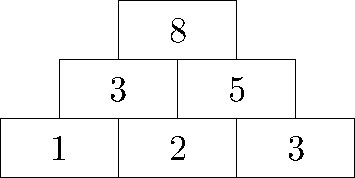
\includegraphics[scale=0.8]{pyramid}
\end{figure}

However, I am not interested in completing the pyramid -- instead, I would much rather go underground.
Thus, for a sequence of $n$ non-negative integers, I will write down a sequence of $n+1$ non-negative integers below it such that each number in the original sequence is the sum of the two numbers I put below it.
However, there may be several possible sequences or perhaps even none at all satisfying this condition.
So, could you please tell me how many sequences there are for me to choose from?

\section*{Input}
The input consists of:
\begin{itemize}
	\item one line with the integer $n$ ($1 \le n \le 10^6$), the length of the base sequence.
	\item one line with $n$ integers $a_1, \dots, a_n$ ($0 \le a_i \le 10^8$ for each $i$), forming the base sequence.
\end{itemize}

\section*{Output}
Output a single integer, the number of non-negative integer sequences that would have the input sequence as the next level in a number pyramid.
